  ATLAS HL-LHC precision physics program will require more statistics, but also increased accuracy in the simulation and reconstruction of ATLAS physics objects. Preliminary ATLAS projections of computing resources (CPU and storage) show significant deficits starting at the beginning of Run 4 (Figure~\ref{fig:2018Res}). If not addressed, these deficits would likely limit ATLAS physics reach.
  
 The goals of this ATLAS Conceptual Design Report (CDR) for HL-LHC Computing are to:
\begin{enumerate}
    \item Establish a baseline computing model, data rates, computing and storage projections for Run 4 and Run 5, including the evolving roles of the Computing Centers,
    \item Establish anticipated cost drivers and infrastructure assumptions,
    \item Outline technological risks and major areas of R\&D.
\end{enumerate}

\begin{figure}[htb!]
  \centering
  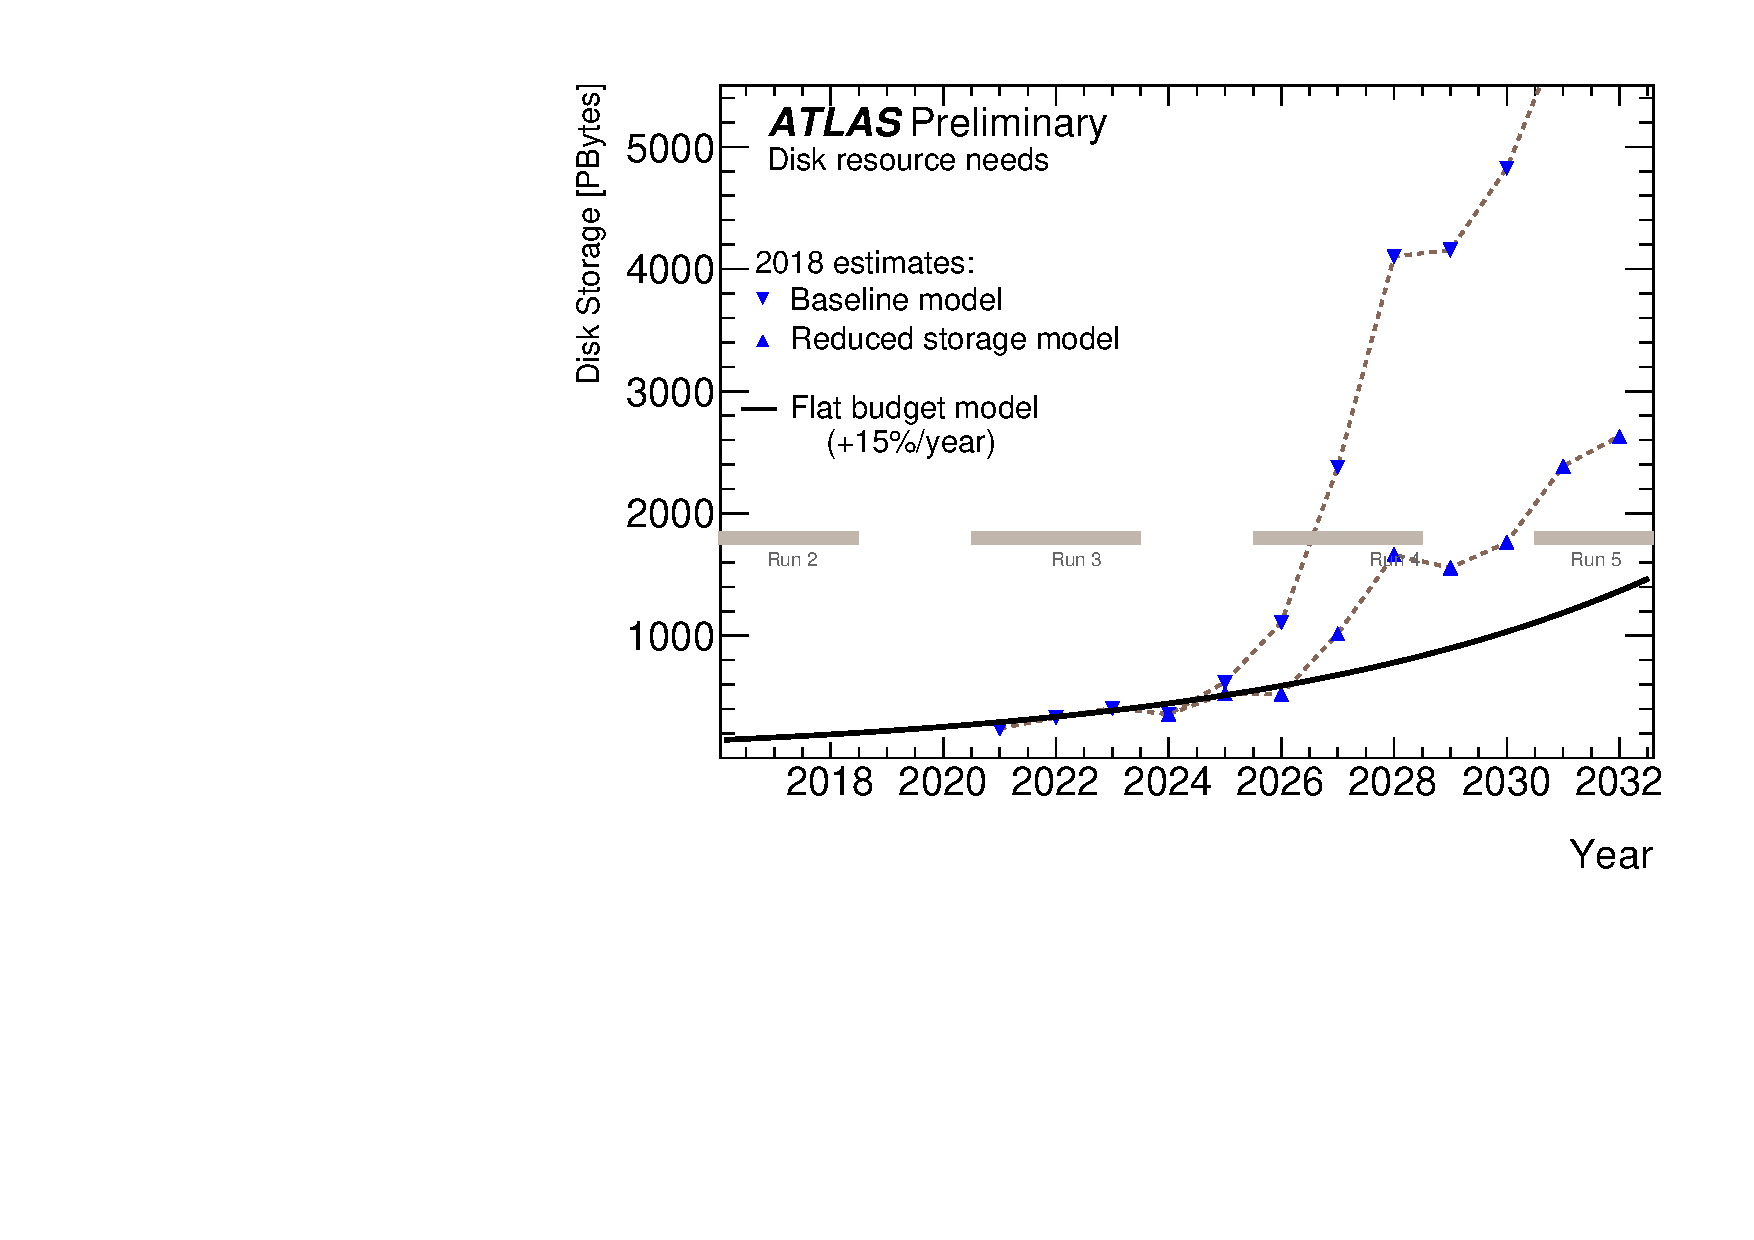
\includegraphics[width=0.48\textwidth]{figures/diskHLLHC_2018.pdf}
  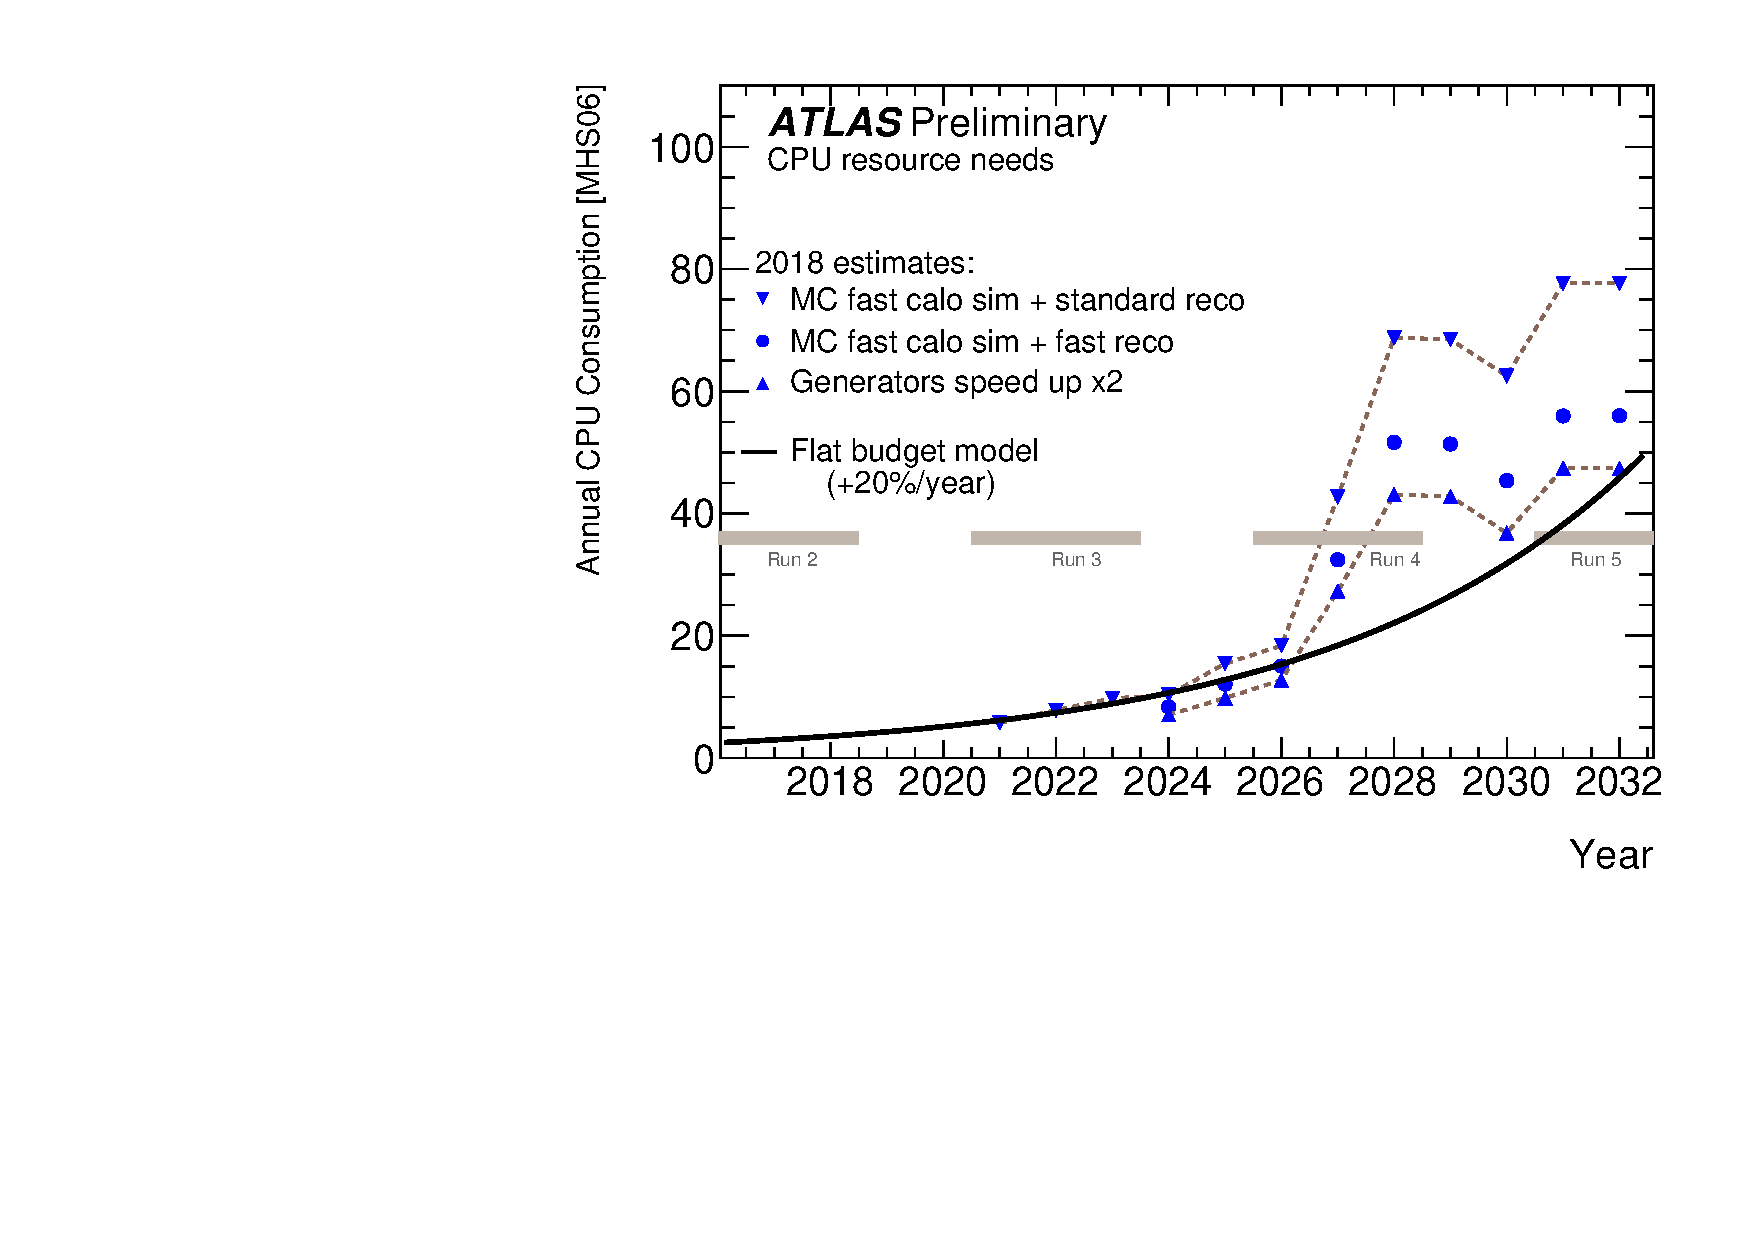
\includegraphics[width=0.50\textwidth]{figures/cpuHLLHC_2018.pdf}
  \caption{ 
Estimated total resources needed for the years 2018 to 2032 for both data and simulation processing {\bf Left:} Disk (in PBytes)  {\bf Right:} CPU (in MHS06).}
  \label{fig:2018Res}
\end{figure}


The CDR process started in the Fall 2019 by reaching out to the ATLAS Computing, Software, and Upgrade Physics communities. This document reflects their input on R \& D priorities and ideas, and on the expected impact of projected storage and computing resource shortages on the HL-LHC Physics program.  It is organized along the traditional ATLAS Computing and Software domains (e.g. core software, simulation, distributed computing, analysis, etc.). 

The document attempts to evaluate the impact on resources and physics reach of the experiment under three scenarios:
\begin{description}
  \item[Conservative] HL-LHC Computing Model and Software are an incremental evolution of the Run 3 one. This would include e.g. 30\% storage savings deriving from the Run 3 Analysis Model \cite{ref:AMSG3}.
  \item[Baseline] Assume success of well-established R\&D projects, e.g. using FastCaloSim \cite{ref:FastChain} for 75\% of MC simulated events, or direct-from-tape processing\cite{ref:DataCarousel}.
  \item[Aggressive] Assume success of one or more "paradigm-shift" R\&D initiatives, such as accurate, fast detector simulation\cite{ref:CaloGAN} that we use to produce 90\% of our simulated events.
\end{description}
 It provides updated estimates of ATLAS computing resource needs under the three scenarios. 

At the end, it describes an initial set of goals and high-level milestones for the ATLAS HL-LHC Computing and Software R\&D program.